\chapter{Physical Implementation and Assembly}

This chapter details the transition from the digital design environment to the physical realization of the OMNICAR platform. The process encompasses the additive manufacturing of the structural components, the integration of the power electronics, and a rigorous multi-stage assembly and validation workflow.

\section{Additive Manufacturing: 3D Printing Phase}

The structural integrity of OMNICAR is primarily based on components manufactured through Fused Deposition Modeling (FDM). All custom parts were produced using a \textbf{Prusa MK3S+} 3D printer, known for its reliability and dimensional accuracy. 

The material selected for the entire chassis and support system was \textbf{PLA (Polylactic Acid)}, chosen for its ease of printing, rigidity, and minimal warping. To balance structural strength with weight optimization, a standard \textbf{infill density of 15\%} was applied to most components. However, for the primary structural elements—specifically the \textbf{Layer 1 Front}, \textbf{Layer 1 Back}, and \textbf{Layer 2}—the infill was increased to 25\% to ensure higher mechanical resistance to the stresses generated by the four DC motors and the overall payload.

\subsection{Printing Statistics and Material Consumption}

The manufacturing process was planned to optimize time and material usage. Table \ref{tab:printing_stats} summarizes the printing time and material consumption (in grams) for the main structural modules, as derived from the G-code analysis.

\begin{table}[H]
\centering
\caption{OMNICAR 3D Printing Parameters and Statistics}
\label{tab:printing_stats}
\rowcolors{2}{gray!10}{white}
\begin{tabularx}{\textwidth}{X c c c}
\toprule
\textbf{Component} & \textbf{Printing Time} & \textbf{Material [g]} & \textbf{Infill [\%]} \\ 
\midrule
Layer 1 Front               & 11h 54m & 115g & 25\% \\
Layer 1 Back                & 9h 47m  & 95g  & 25\% \\
Layer 2                     & 6h 41m  & 70g  & 25\% \\
Battery Case and Support    & 7h 11m  & 55g  & 15\% \\
Structural Pillars (Set)    & 6h 29m  & 88g  & 15\% \\
Stand                       & 19h 44m & 160g & 15\% \\
\midrule
\textbf{TOTAL}              & \textbf{61h 46m} & \textbf{583g} & \textbf{---} \\
\bottomrule
\end{tabularx}
\end{table}

\begin{figure}[H]
    \centering
    \begin{minipage}[b]{0.49\textwidth}
        \centering
        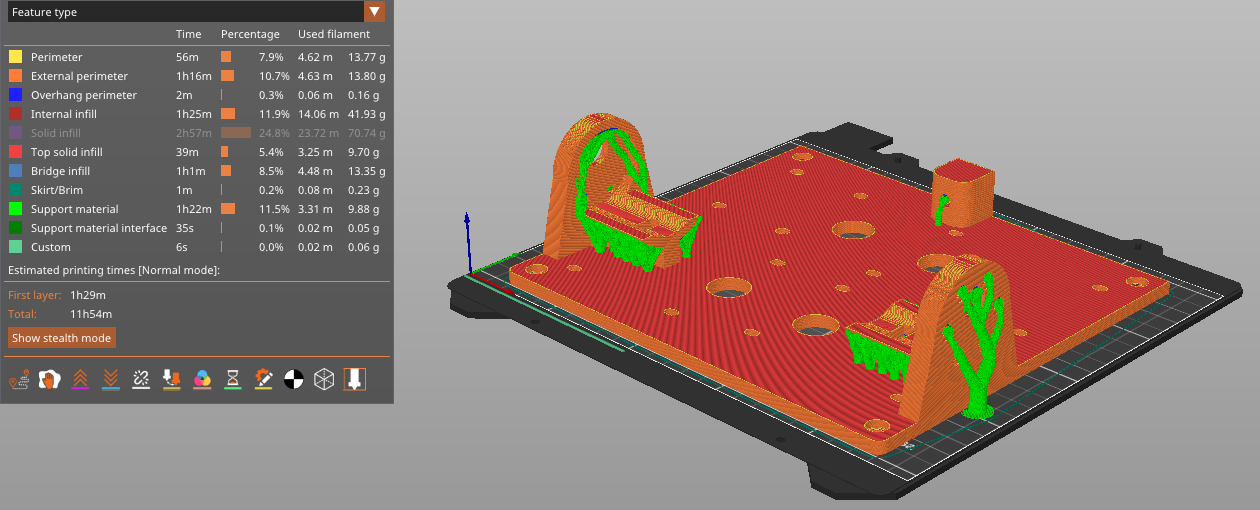
\includegraphics[width=\textwidth]{IMG/PrusaSlicer/prusa_ly1_front.png}
        \caption*{Front lower layer}
    \end{minipage}
    \hfill
    \begin{minipage}[b]{0.49\textwidth}
        \centering
        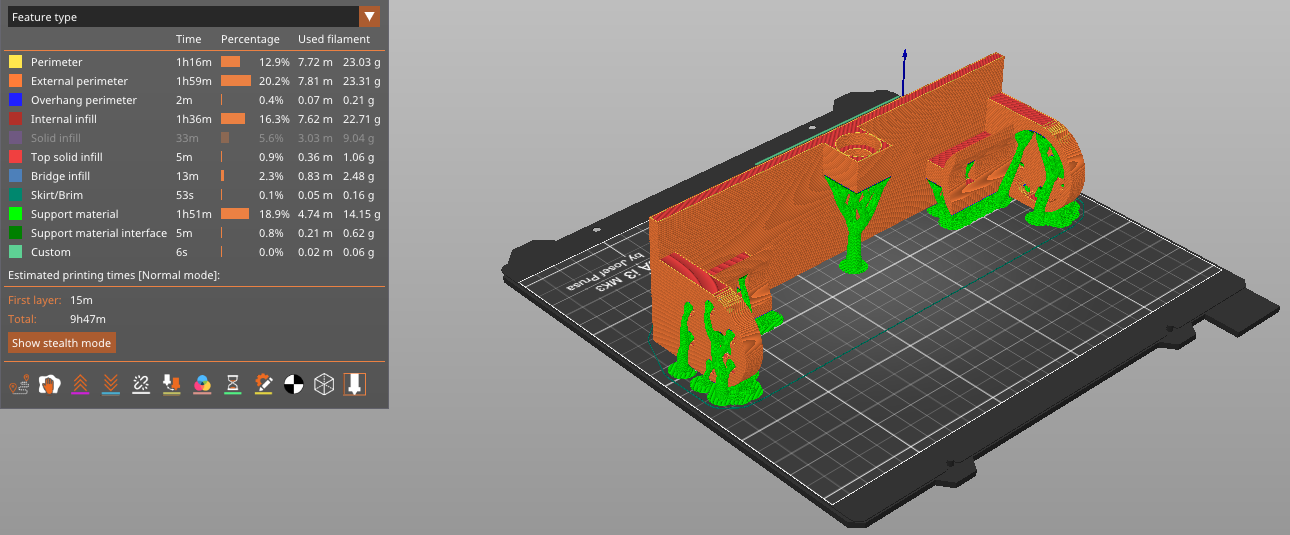
\includegraphics[width=\textwidth]{IMG/PrusaSlicer/prusa_ly1_back.png}
        \caption*{Back lower layer}
    \end{minipage}

    \vspace{1em} 

    \begin{minipage}[b]{0.49\textwidth}
        \centering
        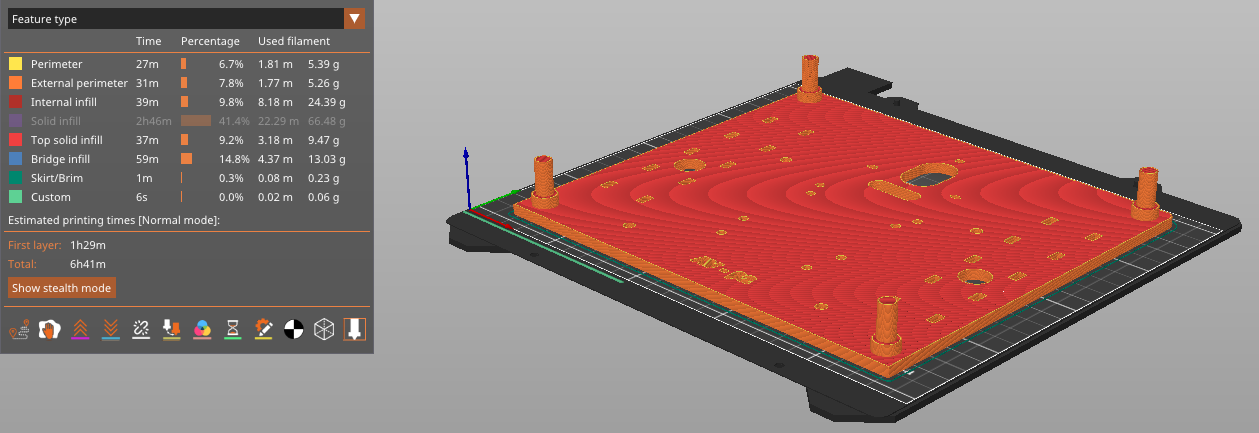
\includegraphics[width=\textwidth]{IMG/PrusaSlicer/prusa_ly2.png}
        \caption*{Upper Layer}
    \end{minipage}
    \hfill
    \begin{minipage}[b]{0.49\textwidth}
        \centering
        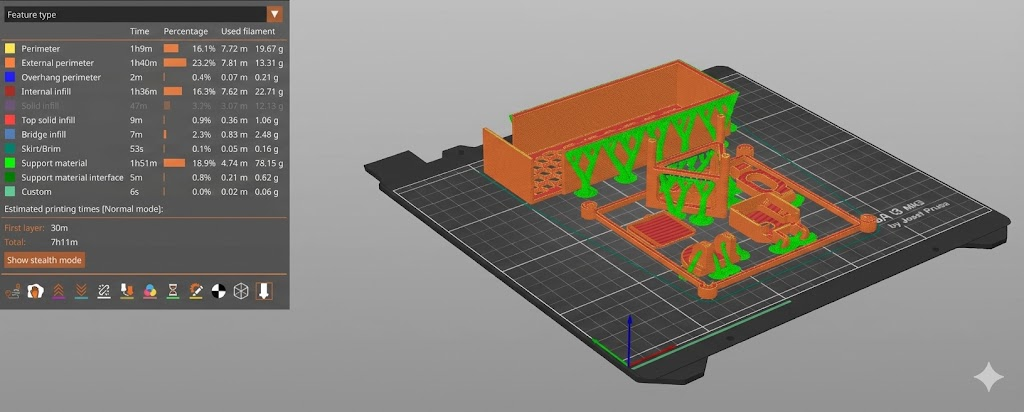
\includegraphics[width=\textwidth]{IMG/PrusaSlicer/Batteria_cover_and_supporti.jpg}
        \caption*{Battery Case and Supports}
    \end{minipage}

    \vspace{1em} 

    \begin{minipage}[b]{0.49\textwidth}
        \centering
        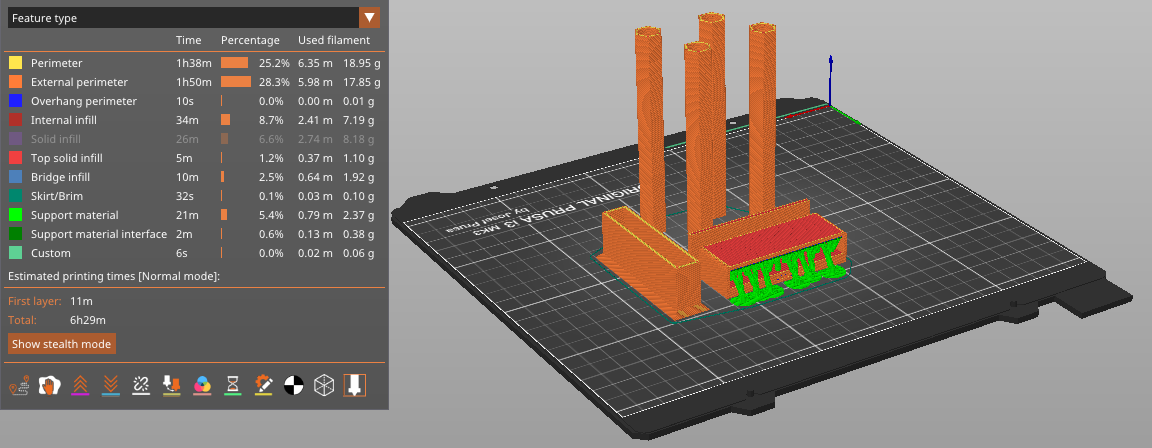
\includegraphics[width=\textwidth]{IMG/PrusaSlicer/prusa_pillar_wago.png}
        \caption*{Structural pillars and Wago Case}
    \end{minipage}
    \hfill
    \begin{minipage}[b]{0.49\textwidth}
        \centering
        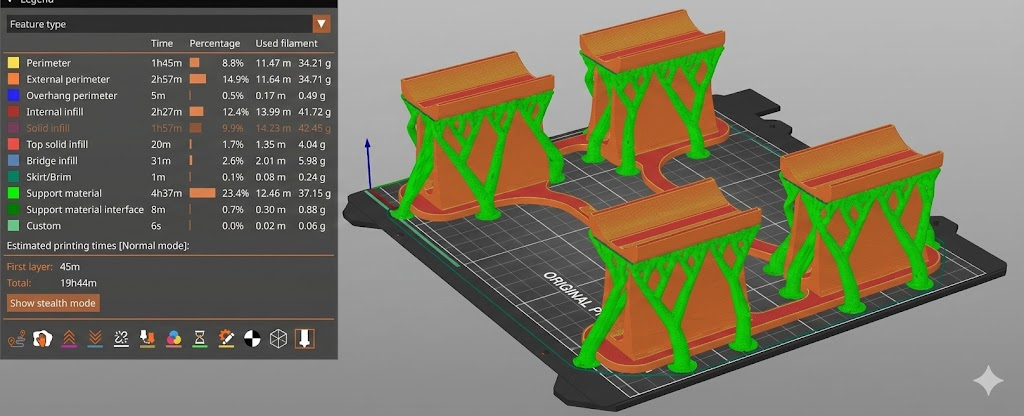
\includegraphics[width=\textwidth]{IMG/PrusaSlicer/Stand_support.jpg}
        \caption*{Robot Test Stand}
    \end{minipage}

    \caption{Slicing preview of OMNICAR components in PrusaSlicer}
    \label{fig:Slicing_preview}
\end{figure}

\section{Mechanical Assembly}

The robot's construction follows a modular "bottom-up" methodology, designed to optimize internal volume distribution and ensure high maintainability. The structure is organized into two primary functional layers connected by rigid vertical pillars.

\subsection{Layer 1: Traction and Power Distribution}
The lower deck (Layer 1) serves as the structural foundation and houses the high-power components. During the initial assembly phase, the motors and core components were positioned without wiring to verify dimensional fits (Figure \ref{fig:physical_assembly_steps}).
\begin{itemize}
    \item \textbf{Suspension and Chassis Coupling:} The connection between the front and rear sections is achieved through a structural bolt passing through flanged bearings. This assembly creates a pivot point that acts as a passive suspension system, allowing the frame to adapt to surface irregularities.
    \item \textbf{Actuation System:} Motor leads were extended by soldering custom wires insulated with heat-shrink tubing to reach the drivers efficiently.
\end{itemize}

\subsection{Power Management: DC-DC Conversion}
To provide a stable logic supply, a \textbf{DC-DC 9A 300W Step-Down Buck Converter} was integrated. The module was calibrated by adjusting its internal multi-turn potentiometer. Although the nominal target was 5.2V to compensate for voltage drops under load, the tuning phase was critical to ensure the Raspberry Pi 5 receives a consistent voltage within its operational tolerances.

\subsection{Layer 2: Logic and Navigation}
The electronics deck (Layer 2) isolates sensitive logic components from electromagnetic interference (EMI). 
\begin{itemize}
    \item \textbf{Processing Unit:} The \textbf{Raspberry Pi 5} is mounted as the central controller.
    \item \textbf{Sensors:} The \textbf{Pi Camera} and \textbf{Lidar} provide an unobstructed $360^{\circ}$ field of view.
\end{itemize}

\begin{figure}[H]
    \centering
    \begin{minipage}[b]{0.40\textwidth}
        \centering
        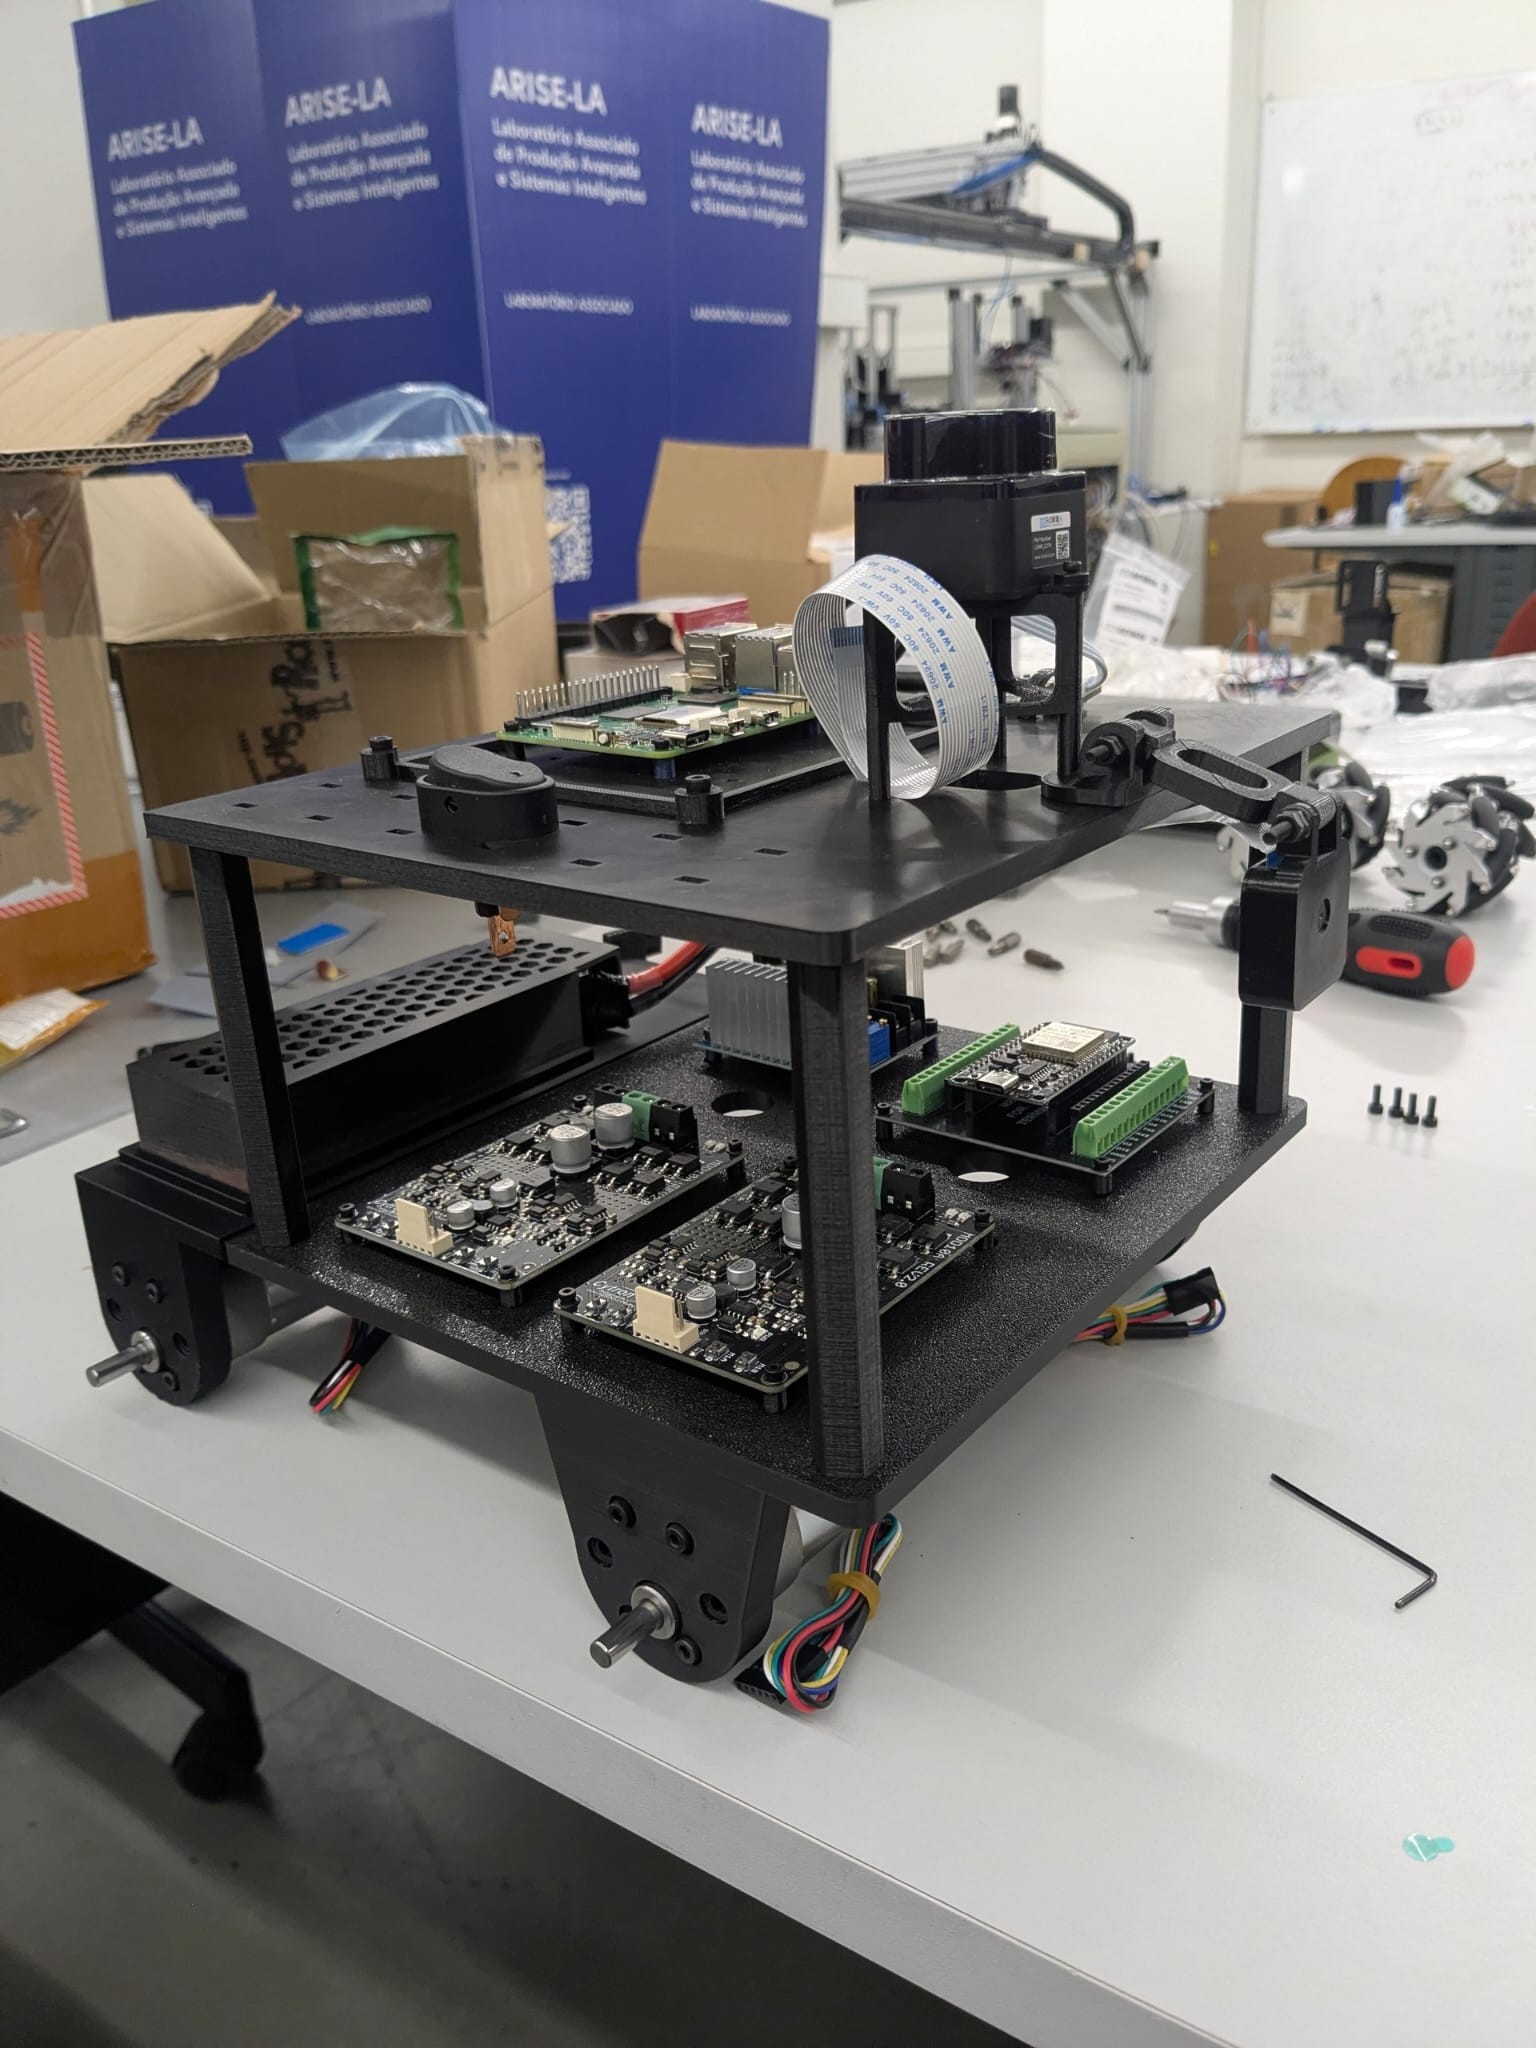
\includegraphics[width=\textwidth]{IMG/Real/Real_omnicar_beta.jpg}
        \caption*{Robot without wiring}
    \end{minipage}
    \hfill
    \begin{minipage}[b]{0.55\textwidth}
        \centering
        \includegraphics[width=\textwidth]{IMG/Real/Real_omnicar_section.jpg}
        \caption*{Main component in the lower layer}
    \end{minipage}
    \caption{Physical assembly of the OMNICAR lower layer}
    \label{fig:physical_assembly_steps}
\end{figure}

\section{Assembly Workflow and System Validation}

The implementation followed a rigorous chronological sequence to minimize the risk of electrical failure and ensure the correctness of the low-level control loops.

\subsection{Wiring and Electrical Pre-testing}
Following the layout of Layer 1 and Layer 2, the wiring was executed according to the previously defined electrical schematic. The circuit was powered by the LiPo battery, and the \textbf{DC-DC converter tuning} was performed as the first step.

The motor actuation was validated by connecting the motors to the MDD10A drivers and supplying 12V for power and 5V for logic. Initial functionality was confirmed \textbf{manually} via the physical test buttons on the drivers, ensuring the gearmotors responded correctly before involving the microcontroller. Subsequently, the DIR and PWM signal lines were routed to the \textbf{ESP32}.

\subsection{Firmware Configuration and Signal Analysis}
A preliminary firmware was developed using \textbf{PlatformIO} to test the PWM generation. As illustrated in Figure \ref{fig:pwm_signal}, the ESP32 successfully generated a stable square wave with a 50\% duty cycle, confirming the correct configuration of the LEDC hardware peripherals.


\begin{figure}[H]
    \centering
    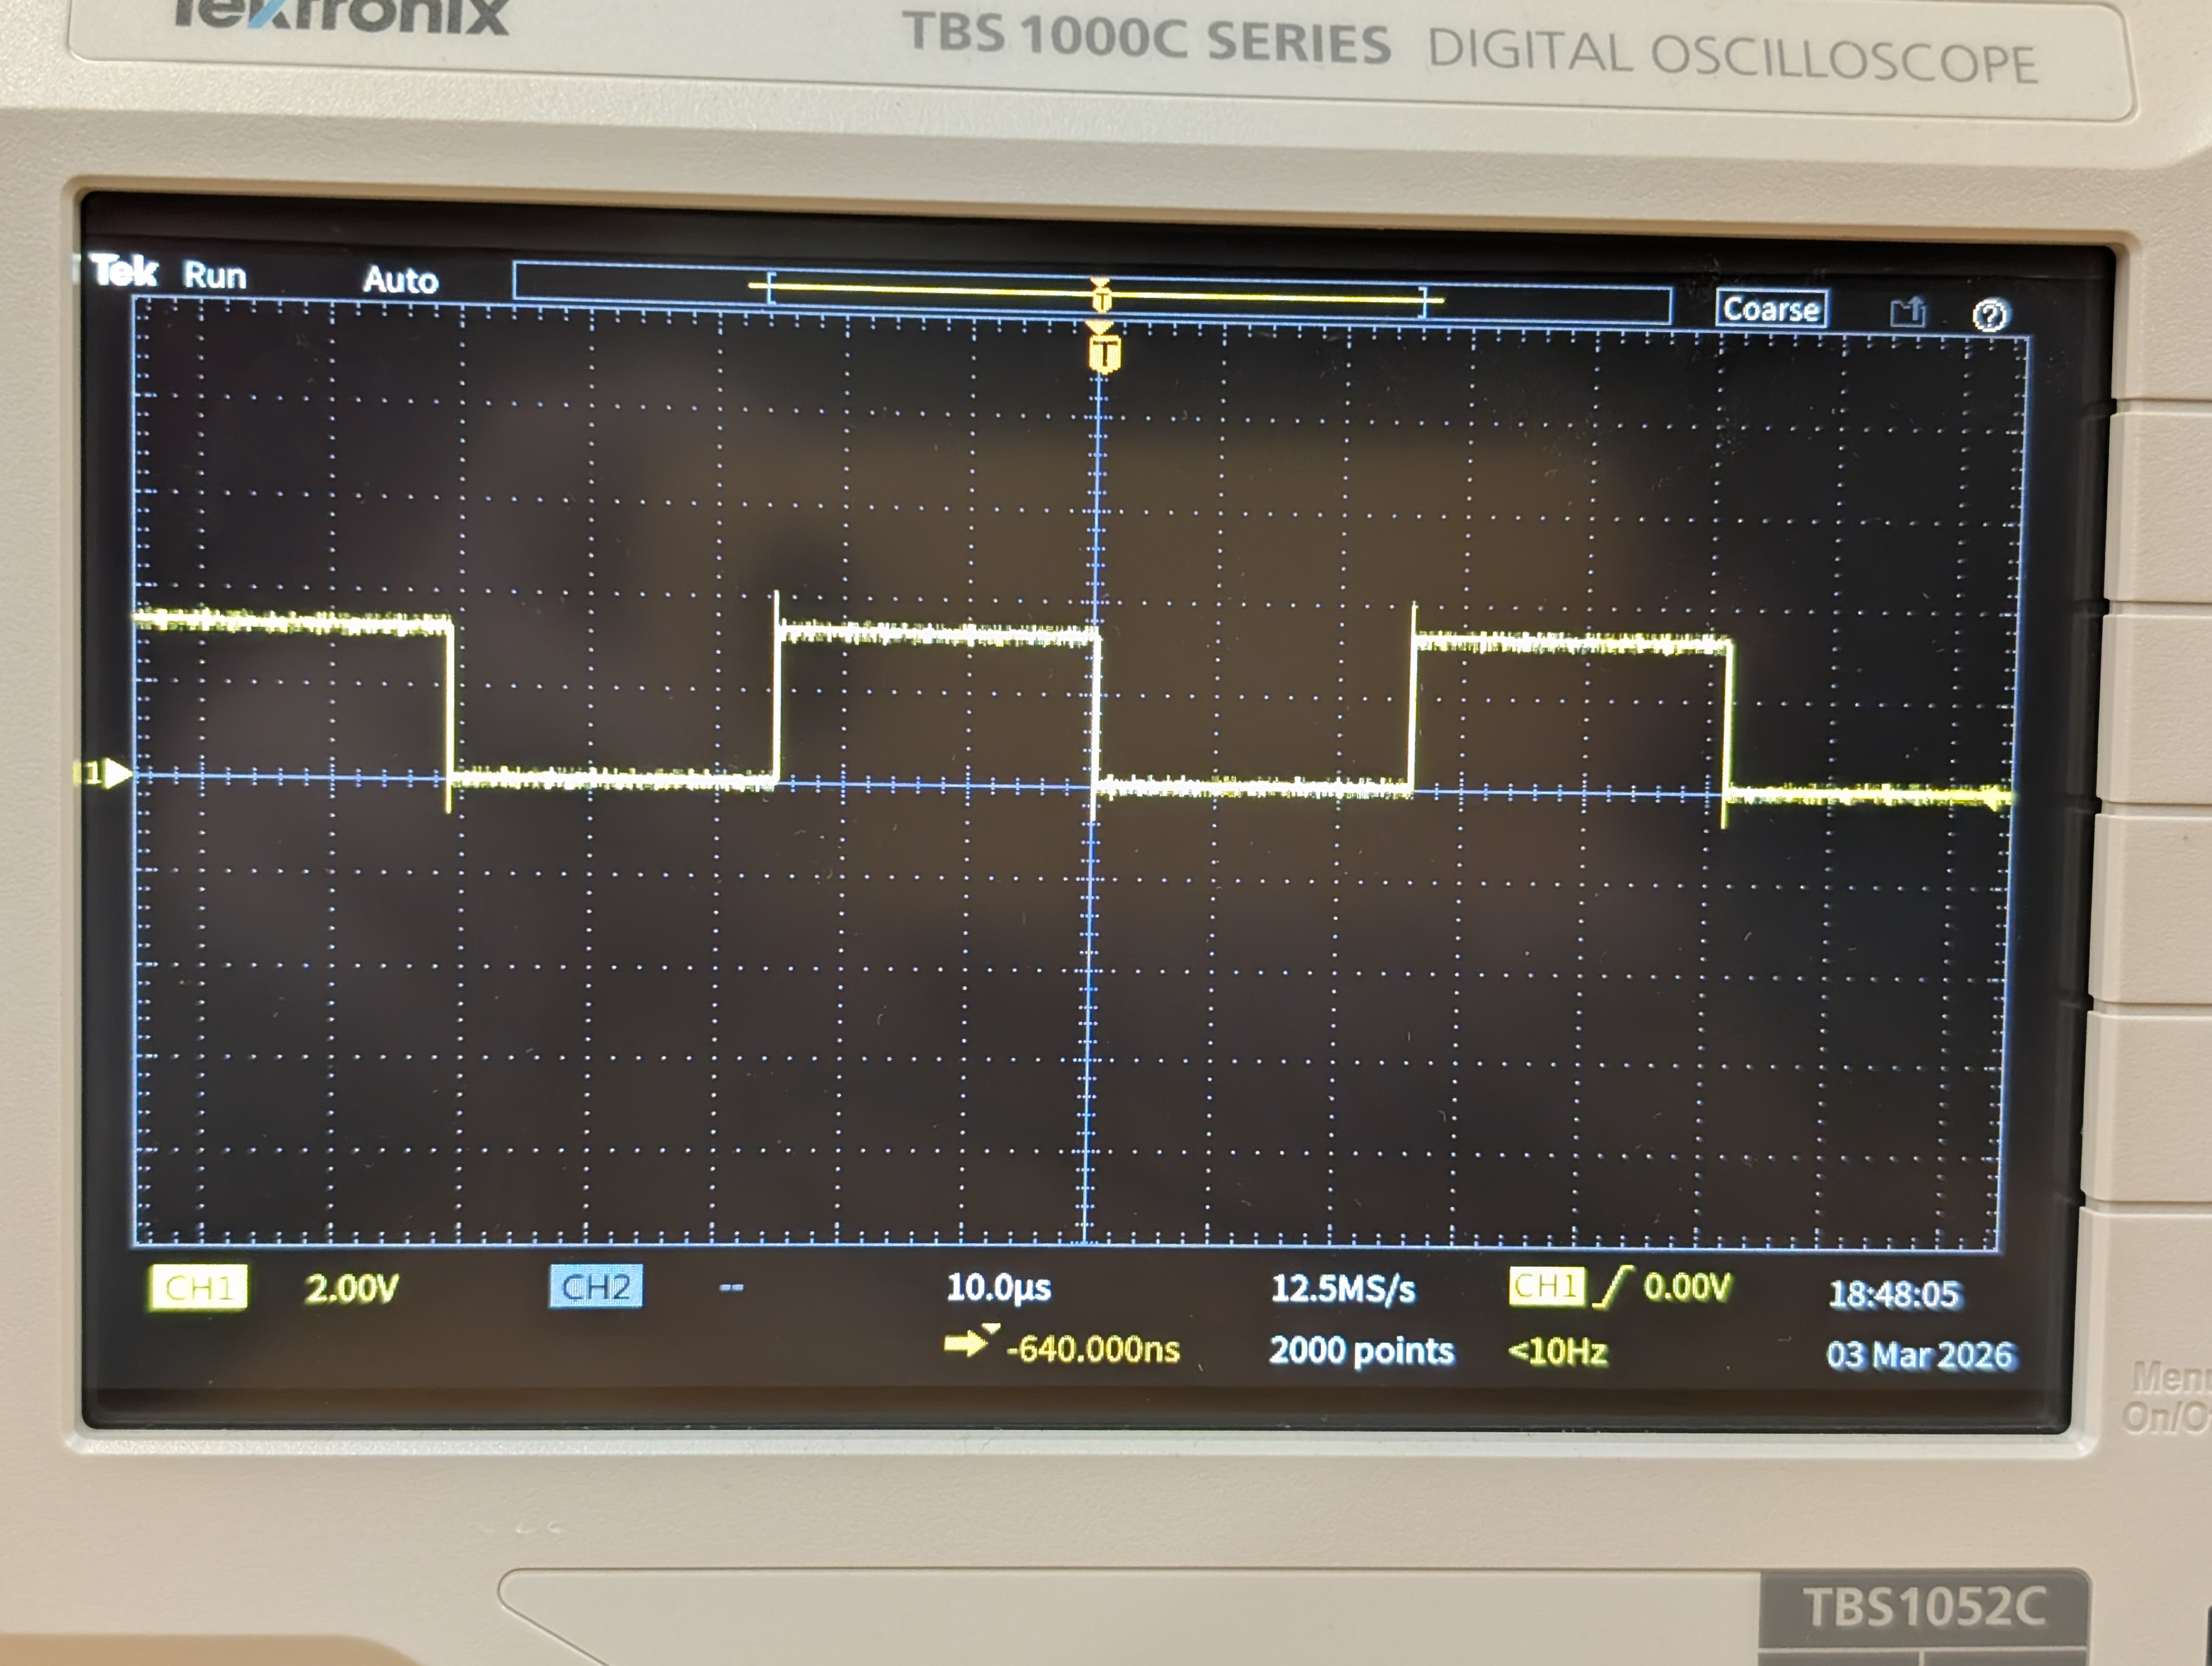
\includegraphics[width=0.45\textwidth]{IMG/Real/PWM_signal.jpg}
    \caption{Oscilloscope capture of the PWM control signal (50\% Duty Cycle)}
    \label{fig:pwm_signal}
\end{figure}

\subsection{Encoder Integration and Signal Conditioning}
The final phase of the assembly involved the integration of the motor encoders. Given that the encoders were powered at 5V, it was necessary to ensure the output signals were compatible with the ESP32's 3.3V logic level. To achieve this, a custom signal conditioning board was realized by soldering \textbf{10k$\Omega$ pull-down resistors} on a prototyping PCB for all 8 encoder channels (A/B phases for 4 motors). This setup, shown in Figure \ref{fig:pulldown_logic}, effectively clamped the input signal to approximately \textbf{3.4V}.

\begin{figure}[H]
    \centering
    \begin{minipage}[b]{0.63\textwidth}
        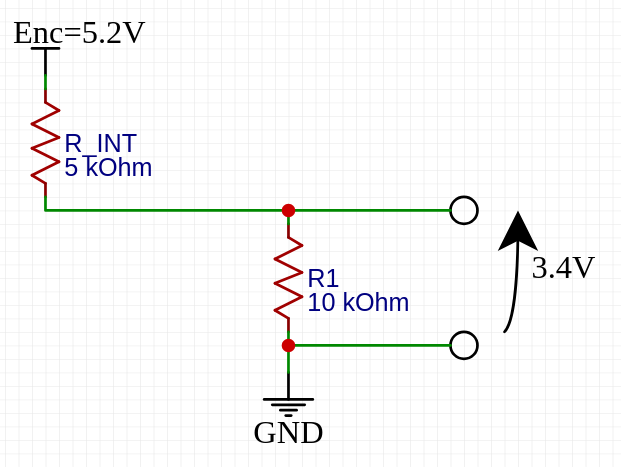
\includegraphics[width=0.6\textwidth]{IMG/Real/pulldown_resistor.png}
        \caption{Pull-down resistor implementation for signal conditioning }
        \label{fig:pulldown_logic}
        \end{minipage}
        \hfill
    \begin{minipage}[b]{0.32\textwidth}
        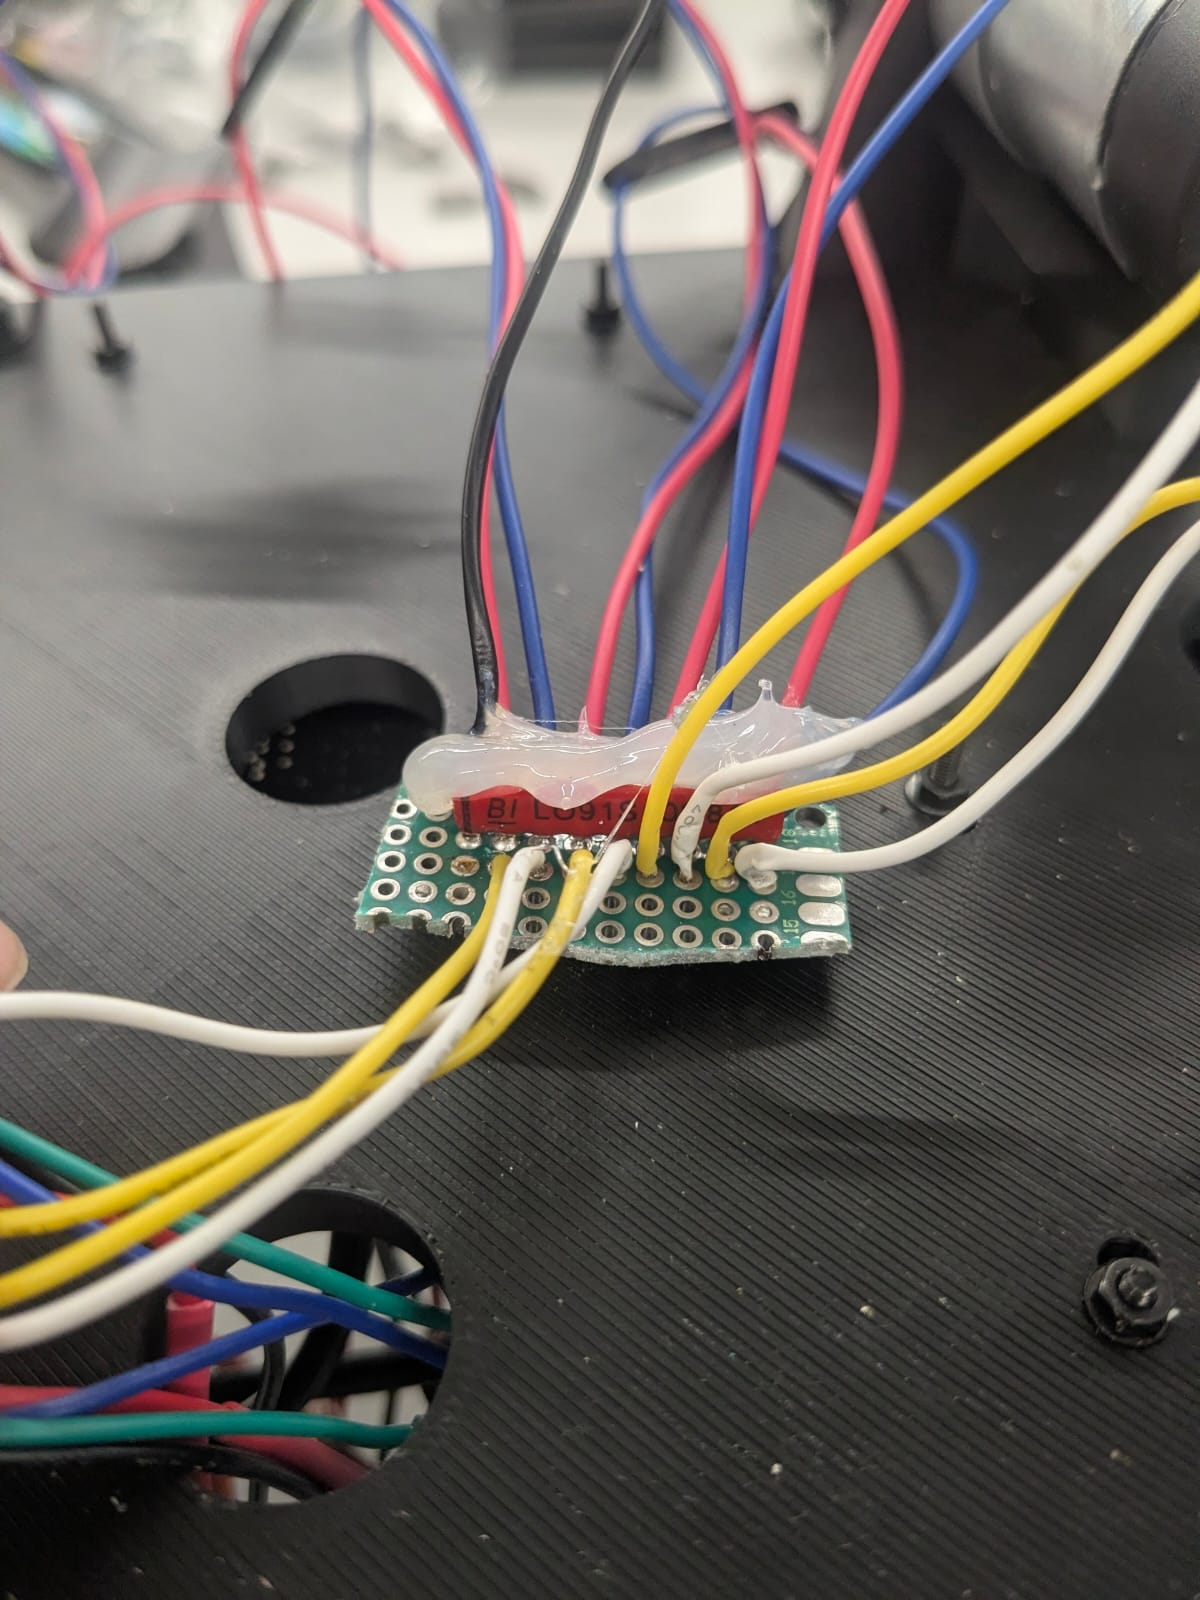
\includegraphics[width=0.6\textwidth]{IMG/Real/pulldown_real.jpeg}
        \caption{Real application of Pull-down resistor}
        \label{fig:pulldown_logic_Real}
        \end{minipage}
    \caption{Solution for Encoder signal}
    \label{fig:Solution for Encoder signal}
\end{figure}

The resulting waveforms were verified via oscilloscope for both forward and backward rotations (Figure \ref{fig:encoder_signals}). The quadrature relationship between the signals remained consistent, providing the high-resolution feedback required for accurate odometry.

\begin{figure}[H]
    \centering
    \begin{minipage}[b]{0.48\textwidth}
        \centering
        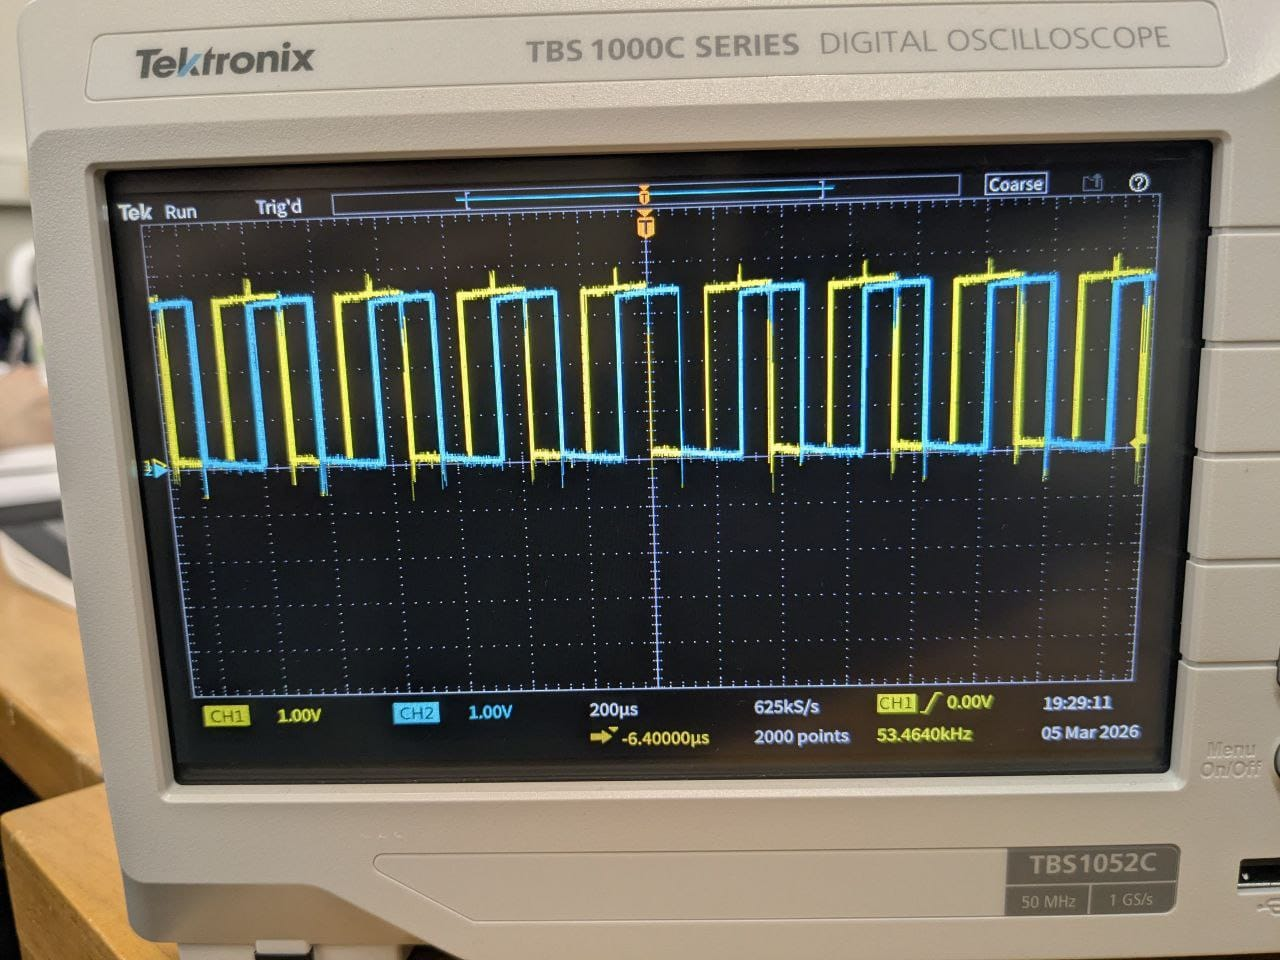
\includegraphics[width=\textwidth]{IMG/Real/encoder_forward.jpeg}
        \caption*{Forward rotation signal}
    \end{minipage}
    \hfill
    \begin{minipage}[b]{0.48\textwidth}
        \centering
        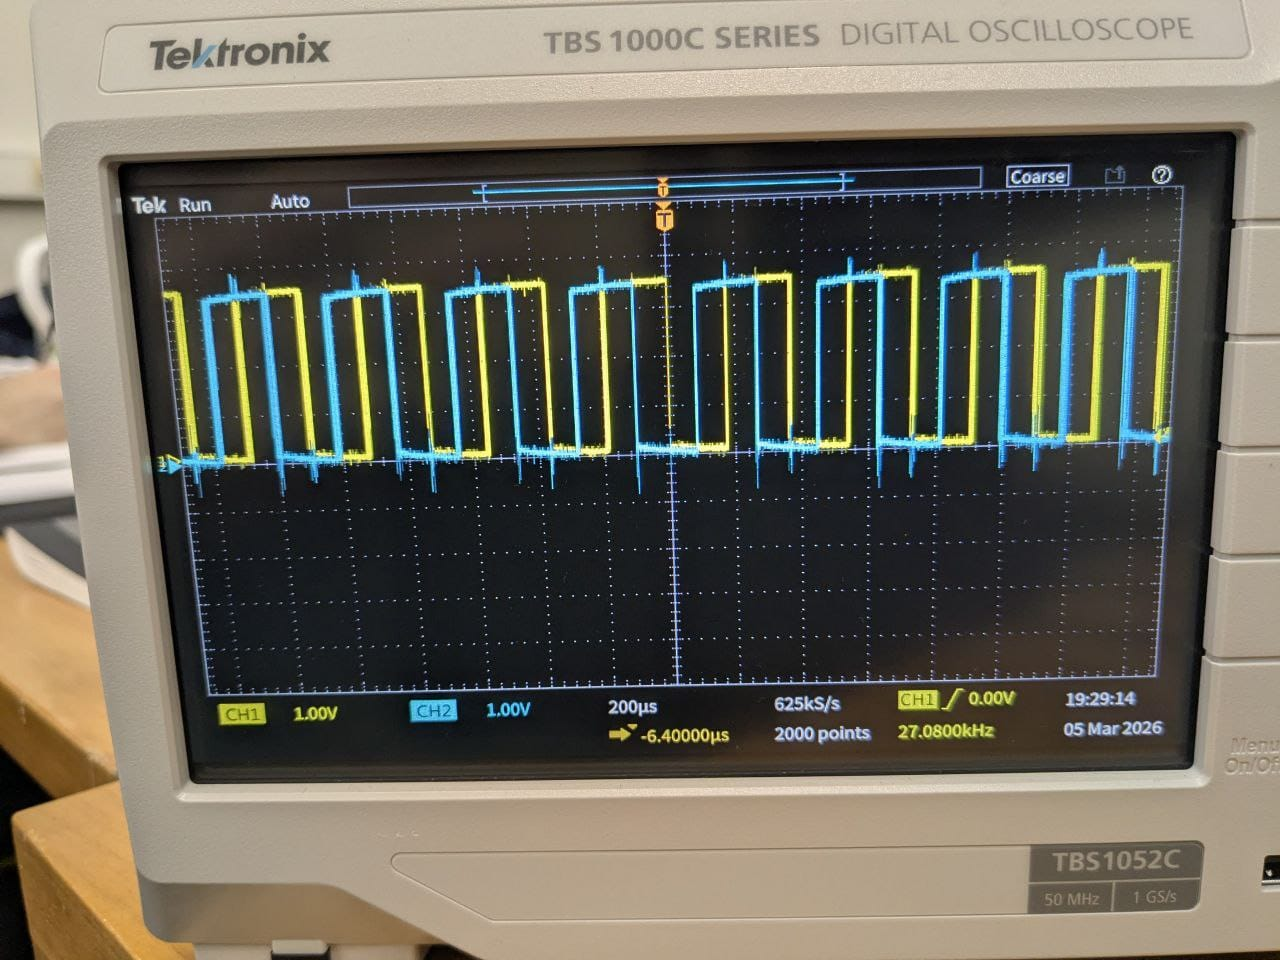
\includegraphics[width=\textwidth]{IMG/Real/encoder_backward.jpeg}
        \caption*{Backward rotation signal}
    \end{minipage}
    \caption{Conditioned encoder signals (approx. 3.4V peak-to-peak)}
    \label{fig:encoder_signals}
\end{figure}

The completion of these hardware validation steps allowed for the commencement of the first dynamic field tests on the integrated platform.

\begin{figure}[H]
    \centering
    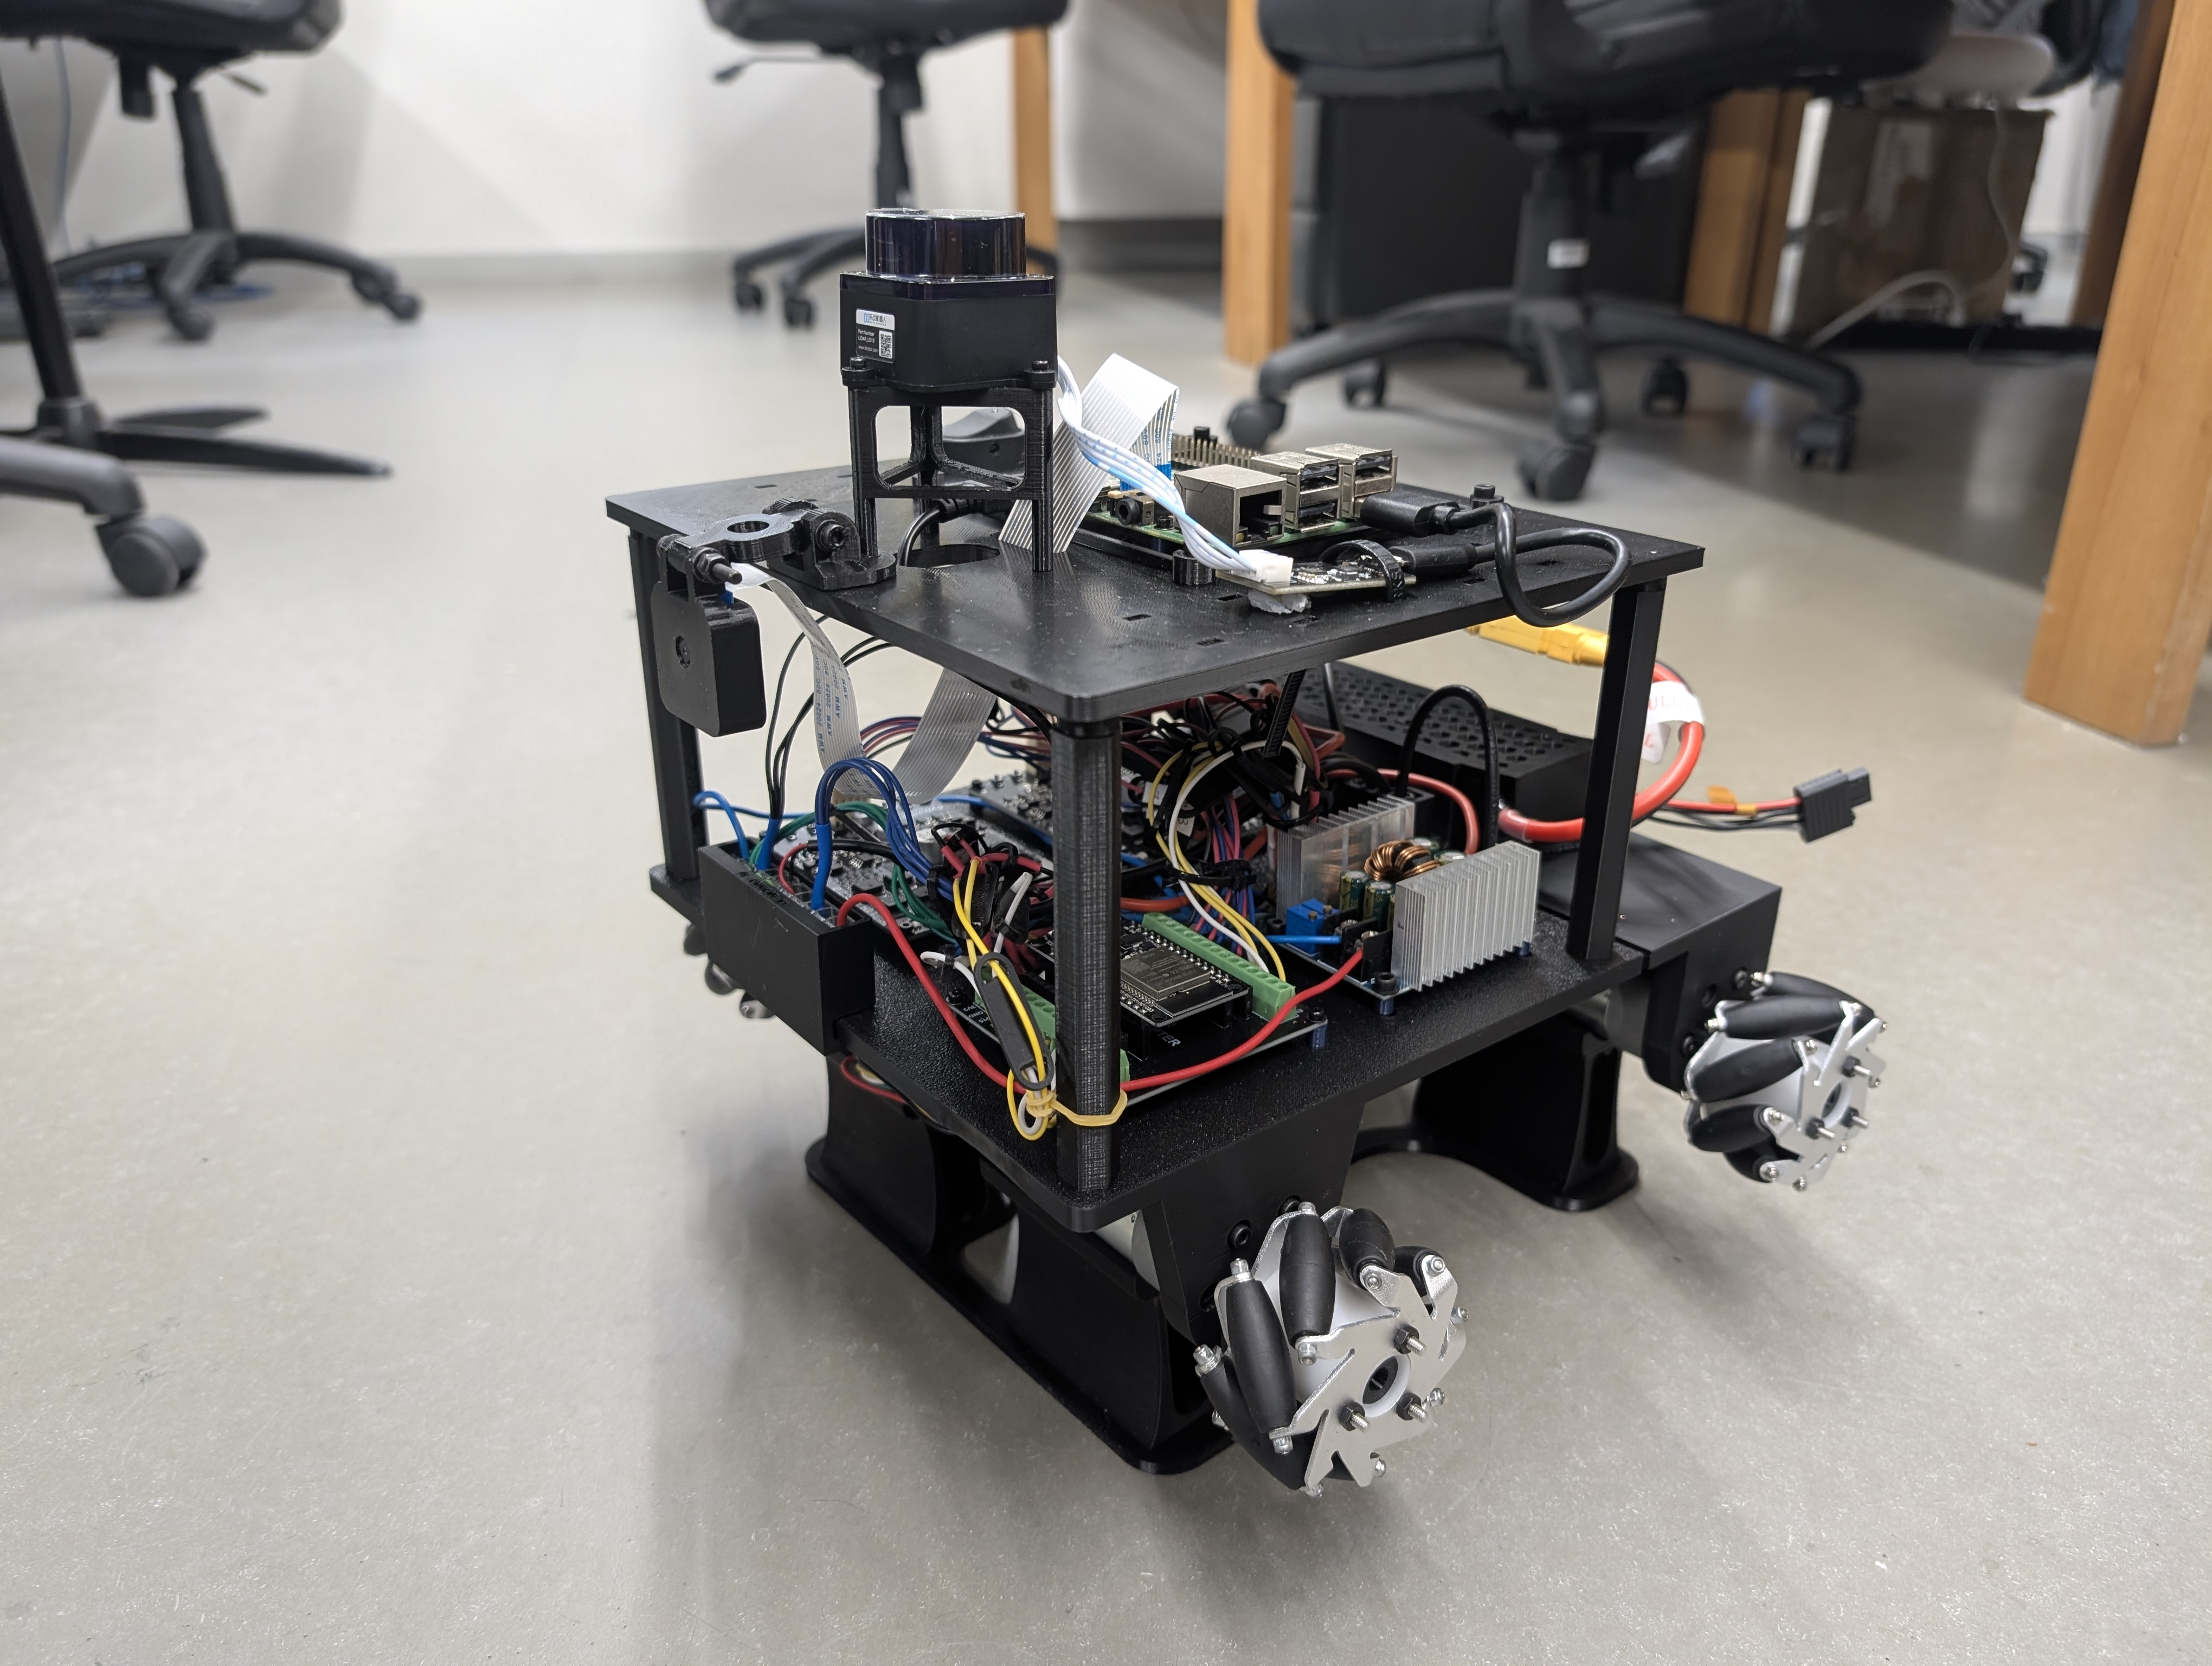
\includegraphics[width=0.7\textwidth]{IMG/Real/Real_omnicar_2.jpg}
    \caption{Fully assembled OMNICAR platform ready for field testing}
    \label{fig:final_robot}
\end{figure}